\NeedsTeXFormat{LaTeX2e}[2005/12/01]

\documentclass[master,
               oneside,
               BCOR10mm,
               ngerman,
               english,
               %final,          %% Endversion; draft fuer schnelles Kompilieren
               ]{GAUBM}

\usepackage{graphicx}
%\usepackage{fancyhdr}
%\usepackage{subcaption}
\usepackage{float}
\usepackage{placeins}
\usepackage{wrapfig} 
%\usepackage{tocloft}
\usepackage{setspace}
\usepackage{babel}
\usepackage{calc}
\usepackage[T1]{fontenc}
\usepackage[utf8]{inputenc}
\usepackage{subfigure} % important
\usepackage{amsmath,amssymb}

\usepackage{lmodern}

\usepackage[comma,numbers,sort&compress]{natbib}


\bibliographystyle{bthesis}

\usepackage{longtable}
%\usepackage[it, bf]{caption}
\usepackage{amsfonts}
\usepackage{amsmath}
\usepackage{mathrsfs}
\usepackage{epsfig}
%\usepackage[clearempty]{titlesec}
\usepackage{booktabs}
\usepackage{hhline}
\usepackage{array}
\usepackage{floatflt}
\usepackage{graphicx}
\usepackage{dcolumn}
\usepackage{bm}
\usepackage{mathrsfs} 
\usepackage{amssymb}
\usepackage{siunitx}

\usepackage{amsfonts}
\usepackage{amsmath}
\usepackage{mathrsfs}
\usepackage{xspace}
%

\sisetup{
  inter-unit-product 	=	$\cdot$,
  fraction-function   	= 	\nicefrac,
  load-configurations 	= 	abbreviations,
  per-mode            	= 	fraction,
  separate-uncertainty	=	true,
  output-decimal-marker	=	{.}
  }
\DeclareSIUnit\barn{b}
\usepackage{float}


\setlength{\oddsidemargin}{0cm}
\setlength{\evensidemargin}{0cm}
\setlength{\topmargin}{-1cm}
\setlength{\textheight}{23cm}
\setlength{\textwidth}{16cm}
\setlength{\parindent}{0cm}

\pagestyle{headings}

\renewcommand{\sectfont}{\bfseries\rmfamily}
\renewcommand{\floatpagefraction}{0.7}
\renewcommand{\textfraction}{0.1}

% Experiments
\newcommand{\dzero}      {D\O\xspace}
\newcommand{\cdf}        {CDF\xspace}
\newcommand{\uubar}      {\mbox{$u\bar{u}$}\xspace}
\newcommand{\ddbar}      {\mbox{$d\bar{d}$}\xspace}
\newcommand{\ccbar}      {\mbox{$c\bar{c}$}\xspace}
\newcommand{\ssbar}      {\mbox{$s\bar{s}$}\xspace}
\newcommand{\ttbar}      {\mbox{$t\bar{t}$}\xspace}
\newcommand{\bbbar}      {\mbox{$b\bar{b}$}\xspace}
\newcommand{\wjets}      {\mbox{$W + 4\; jets$}\xspace}
\newcommand{\pttbar}     {\mbox{$p_{t\bar{t}}$}\xspace}
\newcommand{\pwjets}     {\mbox{$p_{W +4 \; jets}$}\xspace}
\newcommand{\ljets}      {\mbox{$\ell$+jets}\xspace}
\newcommand{\ejets}      {\mbox{$e$+jets}\xspace}
\newcommand{\mujets}     {\mbox{$\mu$+jets}\xspace}

% Laboratories
\newcommand{\fermilab}  {{F{\textsc{ermilab}}}\xspace}
\newcommand{\tevatron}  {{T{\textsc{evatron}}}\xspace}
\newcommand{\opal}      {{O{\textsc{pal}}}\xspace}
\newcommand{\cern}      {{C{\textsc{ern}}}\xspace}
\newcommand{\fnal}      {{F{\textsc{nal}}}\xspace}
\newcommand{\atlas}     {{A{\textsc{tlas}}}\xspace}
\newcommand{\lhc}       {{L{\textsc{hc}}}\xspace}
\newcommand{\lhcb}      {{L{\textsc{hc}}}{\scriptsize{b}}\xspace}
\newcommand{\lep}       {{L{\textsc{ep}}}\xspace}
\newcommand{\slc}       {{S{\textsc{lc}}}\xspace}
\newcommand{\pep}       {{P{\textsc{ep}}}\xspace}
\newcommand{\petra}     {{P{\textsc{etra}}}\xspace}
\newcommand{\hera}      {{H{\textsc{era}}}\xspace}
\newcommand{\lepaleph}  {{A{\textsc{leph}}}\xspace}
\newcommand{\delphi}    {{D{\textsc{elphi}}}\xspace}
\newcommand{\leplthree} {{L{\textsc{3}}}\xspace}
\newcommand{\lepopal}   {{O{\textsc{pal}}}\xspace}
\newcommand{\doris}     {{D{\textsc{oris}}}\xspace}
\newcommand{\isr}       {{I{\textsc{sr}}}\xspace}
\newcommand{\desy}      {{D{\textsc{esy}}}\xspace}
\newcommand{\kek}       {{K{\textsc{ek}}}\xspace}
\newcommand{\slac}      {{S{\textsc{lac}}}\xspace}
\newcommand{\tristan}   {{T{\textsc{ristan}}}\xspace}
\newcommand{\cms}       {{C{\textsc{ms}}}\xspace}
\newcommand{\alice}     {{A{\textsc{lice}}}\xspace}
\newcommand{\zeus}      {{Z{\textsc{eus}}}\xspace}
\newcommand{\hone}      {{H{\textsc{1}}}\xspace}
\newcommand{\minuit}    {{M{\textsc{inuit}}}\xspace}
\newcommand{\herwig}    {{H\textsc{erwig}}\xspace}
\newcommand{\acermc}    {{A\textsc{cerMC}}\xspace}
\newcommand{\evtgen}    {{E\textsc{vtgen}}\xspace}
\newcommand{\mcfm}      {{M\textsc{cfm}}\xspace}
\newcommand{\mcatnlo}   {{M\textsc{c@nlo}}\xspace}
\newcommand{\sherpa}    {{S\textsc{herpa}}\xspace}
\newcommand{\jimmy}     {{J\textsc{immy}}\xspace}
\newcommand{\cteq}      {{C\textsc{teq}}\xspace}
\newcommand{\pythia}    {{P\textsc{ythia}}\xspace}
\newcommand{\jetnet}    {{J\textsc{etnet}}\xspace}
\newcommand{\isajet}    {{I\textsc{sajet}}\xspace}
\newcommand{\jetset}    {{J\textsc{etset}}\xspace}
\newcommand{\vecbos}    {{V\textsc{ecbos}}\xspace}
\newcommand{\alpgen}    {{A\textsc{lpgen}}\xspace}
\newcommand{\vegas}     {{V\textsc{egas}}\xspace}
\newcommand{\gnu}       {{G\textsc{nu}}\xspace}
\newcommand{\onetop}    {{O\textsc{neTop}}\xspace}
\newcommand{\ztop}      {{Z\textsc{Top}}\xspace}
\newcommand{\toprex}    {{T\textsc{opRex}}\xspace}
\newcommand{\singletop} {{S\textsc{ingleTop}}\xspace}
\newcommand{\madgraph}  {{M\textsc{adgraph}}\xspace}
\newcommand{\madevent}  {{M\textsc{adevent}}\xspace}
\newcommand{\comphep}   {{C\textsc{omphep}}\xspace}
\newcommand{\qq}        {{Q\textsc{q}}\xspace}
\newcommand{\tauola}    {{T\textsc{auola}}\xspace}
\newcommand{\geant}     {{G\textsc{eant}}\xspace}
\newcommand{\GEANT}     {{G\textsc{eant}}\xspace}
\newcommand{\amegic}    {{A\textsc{megic++}}\xspace}

\newcommand{\met}       {\mbox{$\not\!\!E_{\mathrm{T}}$}\xspace}
\newcommand{\metcal}    {\mbox{$\not\!\!E_{Tcal}$}\xspace}
\newcommand{\MET}       {$\not\!\!E_{\mathrm{T}}$}
\newcommand{\lowmet}    {low-\mbox{$\not\!\!E_{\mathrm{T}}$}-QCD\xspace}
\newcommand{\lumi}      {$\mathcal{L}$\xspace}
\newcommand{\intlumi}   {$\int\mathcal{L}\,\mathrm{d}t$\xspace}

\newcommand{\runi}      {Run~I\xspace}  %% For Tevatron! (Roman numerals)
\newcommand{\runii}     {Run~II\xspace}
\newcommand{\LHCruni}   {Run~1\xspace}  %% For LHC! (Arabic numerals)
\newcommand{\LHCrunii}  {Run~2\xspace}
\newcommand{\LHCruniii}  {Run~3\xspace}

\newcommand{\tabheadfont}[1]{\textbf{#1}}
\usepackage{booktabs}
\usepackage{longtable}
\usepackage{array}

\usepackage{textcomp,gensymb}
\usepackage[colorlinks=false,
            pdfstartview=FitH,
            breaklinks=true,
            bookmarksopen=true,
            bookmarksnumbered=true
            ]{hyperref}
\usepackage{cleveref}


\begin{document}

\ThesisAuthor{Siemen Henning}{Aulich}
\PlaceOfBirth{Emden}
\ThesisTitle{}{Improving Event Reconstruction for Dileptonic Decays of Top Quarks Pairs Using Machine Learning}
\FirstReferee{Prof.~Dr.~Stan Lai}
\Institute{DESY Hamburg}
\SecondReferee{Dr.~Katharina Behr}

\CourseName{M.Phy.1610: Development and Realization of Scientific
Projects in Theoretical Physics}


\ThesisBegin{7}{4}{2025}
\ThesisEnd{4}{12}{2026}

\frontmatter
\maketitle
\cleardoublepage
\begin{abstract}
  Here the key results of the thesis can be presented in about
  half a page.
  \bigskip\par
  \textbf{Keywords:} Physics, Master thesis
\end{abstract}

\cleardoublepage
\mainmatter
\tableofcontents

\chapter{Introduction}
\label{chap:introduction}
The top quark, being the heaviest known elementary particle, plays a crucial role in the Standard Model of particle physics. Its unique properties and interactions make it an excellent probe for testing the limits of our current understanding of fundamental forces and searching for potential new physics beyond the Standard Model. It is one of the most studied processes at the Large Hadron Collider (\lhc) at \cern.
Top quarks are predominantly produced in pairs (\ttbar) via the strong interaction in proton-proton collisions at the \lhc. Each top quark decays almost exclusively into a W boson and a b-quark. The W boson can further decay either leptonically (into a charged lepton and a neutrino) or hadronically (into a pair of quarks). The dileptonic decay channel, where both W bosons decay leptonically, results in a final state with two charged leptons, two b-jets, and two neutrinos. This channel, while having a lower branching ratio compared to other decay modes, offers a cleaner experimental signature due to the presence of high-\pt leptons and reduced hadronic activity. However, the presence of two neutrinos in the final state poses significant challenges for event reconstruction, as they evade detection, leading to missing transverse energy (\met) in the event.

Due to its clean signature and sensitivity to various top quark properties, the dileptonic \ttbar channel is widely used for precision measurements of the top properties or spin correlations. Two recent highlights in top quark physics are the stringent tests of spin correlations and quantum effects in pairs of top quarks, and the observation of a possible quasi-bound state resonance in the $t\bar{t}$ invariant mass spectrum. Both effects are predominantly studied in the dilepton decay channel of the top quark in a mass range close to the $t\bar{t}$ production threshold. The latter presents a very exciting opportunity to extend our current understanding of non-relativistic Quantum Chromodynamics.

Both analyses rely on measurements of angular distributions and correlations between the decay products of the top quarks. Probing this system requires a precise reconstruction of the top quarks, which is complicated by the presence of the two neutrinos. While analytical neutrino regression strategies have been studied extensively, the problem of correctly assigning b-jets to their parent top quarks remains largely unstudied. In the all-hadronic and lepton+jets channels, various methods for jet assignment have been developed and employed successfully. However, in the dileptonic channel, the jet assignment problem was often simplified or overlooked due to a focus on neutrino reconstruction. However, many of the sensitive variables used in $t\bar{t}$ precision measurements depend critically on the correct assignment of the jets. Misassignments can lead to significant biases and degrade the resolution of reconstructed observables, ultimately limiting the precision of measurements.

Inspired by the success of machine learning architectures in tackling the assignment challenge for hadronic decay channels, this work investigates using a transformer model for the dilepton channel. It introduces the necessary theoretical background in \Cref{chap:background} before detailing the use of machine learning in particle physics in \Cref{chap:machine-learning}. The reconstruction methods are outlined in \Cref{chap:reconstruction-methods}, followed by the development of the machine learning-based jet assignment in \Cref{chap:ml-jet-selection}. For this, different transformer architectures are explored and optimized. The performance of the developed methods is evaluated in \Cref{chap:performance-evaluation}, where thee impact on relevant physics observables is assessed. Finally, \Cref{chap:conclusion} summarizes the findings and discusses potential future directions for further improving dileptonic \ttbar event reconstruction.

\chapter{Theoretical Background}
\label{chap:background}
\section{The Standard Model of Particle Physics}
\label{sec:standard_model}
\begin{figure}[h]
    \centering
    \includegraphics[width=0.8\textwidth]{figures/standard_model.pdf}
    \caption{The particles of the Standard Model. Particle porperties taken from Ref. \cite{PDG2024}.}
    \label{fig:standard_model_particles}
\end{figure}
The Standard Model of Particle Physics (SM) provides the theoretical foundation describing three of the four elementary forces as well the particles making up the known matter.\\
The Figure \ref{fig:standard_model_particles} shows a tabular overview of the known particle of the Standard Model.
The SM classifies the elementary particles into fermions and bosons.
Fermions are the building blocks of matter and have half-integer spin values. They are further divided into quarks and leptons.
Quarks experience all four fundamental forces, while leptons do not participate in the strong interaction.
Bosons are the force carriers of the fundamental interactions and have integer spin values.
The photon, W and Z bosons, and gluons mediate the electromagnetic, weak, and strong forces, respectively.
The Higgs boson is responsible for giving mass to other particles through the Higgs mechanism.\\
Based on the coupling of the weak interaction, two particles are grouped into one iso-spin doublet.
The iso-spin is the quantum number related to the weak interaction. Two quarks form one doublet and one lepton and its corresponding neutrino form another doublet.
Based on the different masses, two iso-spin doublets are grouped into what is called a generation.
There are three generations of fermions, with each generation containing heavier particles than the previous one.

\section{Top Quark Physics}
\label{sec:top_quark_physics}
The positive iso-spin partner of the third generation quark doublet is the top quark ($t$). With a mass of about $173\,\mathrm{GeV}/c^2$ \cite{PDG2024}, it is the heaviest known elementary particle.
Due to its high mass, the top quark has a very short lifetime of approximately $5\times10^{-25}\,\mathrm{s}$ \cite{PDG2024}, which is shorter than the timescale for hadronization.


\chapter{Machine Learning in High Energy Physics}
Since this work focuses on improving the event reconstruction of dileptonic \ttbar decays using machine learning techniques, this chapter provides an overview of the fundamental concepts and methodologies employed in machine learning. 

\section{Supervised Learning}
Machine learning can be broadly categorized into supervised and unsupervised learning. In supervised learning, the model is trained on a labeled dataset, where each input data point is associated with a corresponding target output. The goal of the model is to learn a mapping from inputs to outputs, enabling it to make accurate predictions on unseen data.
\subsection{Monte Carlo Training Data}
In high energy physics, supervised learning is commonly performed by training mdoels on simulated datasets. The way the Monte Carlo Event modelling is performed in particle physics, makes it naturally suited for supervised learning tasks.\\
Events are usually simulated using a cascade of different programs, each simulating a different state of the event. First the hard scattering process is simulated using matrix element generators like \textsc{MadGraph} \cite{madevent_1} or \textsc{Powheg} \cite{powheg}. These programs calculate the probabilities of different particle interactions based on the underlying physics theories, such as the Standard Model. Using these probabilities, they generate events that represent the initial state of the particles after the collision. The possible kinematic phase space is sampled according to these probabilities, resulting in a set of particles with specific momenta and energies. This type of event variables is often referred to as \textit{parton-level}.\\
Next, the parton showering and hadronization processes are simulated using programs like \textsc{Pythia} \cite{pythia}. Parton showering models the emission of additional particles from the initial partons, while hadronization simulates the formation of hadrons from quarks and gluons. These processes are crucial for accurately modelling the final state particles observed in detectors.\\
Finally, detector simulation programs like \textsc{Geant4} \cite{geant4} are used to simulate the interaction of particles with the detector material, producing realistic detector responses. This includes simulating the energy deposits in calorimeters, hits in tracking detectors, and other relevant signals.\\
While the actual detector response is simulated using complex detector simulation software, for many machine learning applications, a simplified representation of the detector response is sufficient. This can involve smearing the particle momenta and energies according to the detector resolution, applying efficiency corrections, and simulating the effects of pile-up.\\
This is because, for the reconstruction of the physics objects, such as jets, leptons, and missing transverse energy, highly sophisticated algorithms are used that already take into account the detector effects (Note, that these algortihms may also be machine learning based,). Therefore, the input features for machine learning models can often be derived directly from these reconstructed objects, rather than relying on the raw detector signals. The reconstructed object event variables are called \textit{reco-level}.
\subsection{Training}
During the training phase, the model is presented with a set of input features derived from the reco-level event variables, along with their corresponding target outputs, which are typically derived from the parton-level event variables. The model learns to map the input features to the target outputs by minimizing a loss function that quantifies the difference between the predicted and true values. Common loss functions include mean squared error for regression tasks and cross-entropy \cite{cross-entropy} loss for classification tasks.\\

\chapter{Experimental Setup}
\label{ch:exper_setup}
\section{The LHC}
The Large Hadron Collider (\lhc) at \cern is a synchrotron designed to accelerate protons and lead nuclei. This work focuses on the proton-proton collisions during \LHCrunii. During \LHCrunii from 2015 to 2018, the \lhc operated at a centre of mass energy of $\sqrt{s}=13\,\unit{\tera\electronvolt}$ with an integrated luminosity of $\mathcal{L}_{int}\approx 140\,\unit{\femto\barn^{-1}}$ \cite{ATLAS:2019pzw}.

After completion of \LHCruniii in June 2026 and an operational pause, the \lhc will operate with increased luminosity as the High-Luminosity Large Hadron Collider (HL-\lhc). During this phase, it is planned to accumulate data with an integrated luminosity of $\mathcal{L}=3\,\unit{\atto\barn^{-1}}$ \cite{Aberle:2749422}.
 \section{The Detector}
The \atlas detector is a general-purpose particle detector at the \lhc at \cern. It can roughly be separated into three elements: the inner detector, the calorimeter and the muon spectrometer \cite{atlas_tdr}.
\subsection{The Coordinate System}
The interaction point marks the origin of the \atlas coordinate system. The $z$-axis is orientated along the beamline, the $x$-axis points towards the centre of the \lhc and the $y$-axis points upwards.

Using this convention, several kinematic variables are defined. One of which is the transverse momentum defined as
\begin{align}
    p_T=\sqrt{p_x^2+p_y^2}
\end{align}
Because of the cylindrical shape of the \atlas detector and the cylindrical symmetry of the interactions, the azimuthal angle is used as another variable. The polar angle relative to the $z$-axis can be used to define the pseudorapidity which can also be expressed in terms of the momentum
\begin{align}
    \eta=-\ln\left(\tan\left(\frac{\theta}{2}\right)\right)=\ln\left(\frac{|\vec p|+p_z}{|\vec p|-p_z}\right)\,.
\end{align}
In the ultra-relativistic limit $m\ll |\vec p|$ the pseudorapidity is equal to the rapidity defined as
\begin{align}
    y=\frac{1}{2}\ln\left(\frac{E+p_z}{E-p_z}\right)\,.
\end{align}
These variables are convenient for the usage in the \atlas experiment because $p_T,\phi$, and differences of $\eta$ are invariant under Lorentz-boost along the $z$-axis.
\subsection{The Inner Detector}
\begin{figure}[ht]
    \centering
    \includegraphics[width=0.8\textwidth]{figures/atlas-detector/IDbriefing_figure1.png}
    \caption{Schematic cross-section of the inner detector of the \atlas detector (\copyright\ \cern).}
    \label{fig:inner_det}
\end{figure} \noindent
The inner detector (ID) is the innermost part of the \atlas detector. It is used for tracking charged particles, particle identification, and primary and secondary vertex determination \cite{atlas_tdr}. The ID consists of three different sub-detectors. Their rough structure is depicted in \Cref{fig:inner_det}. The ID is encapsulated with a solenoid magnet providing a $2\,\unit{\tesla}$ axial magnetic field on the inside of the ID. The magnetic field is crucial to measure the momentum of a charged particle. The transverse momentum is measured as the curvature of the particle's track due to the Lorentz force.

The detector part closest to the beam pipe is the pixel detector. It consists of 1744 modules arranged in three barrel layers. Each module hosts 47232 silicon pixels with a size of $50\times 400\,\unit{\micro \metre^2}$. The pixels are semiconductor trackers used to detect the traversing of charged particles.

The following part of the detector is the semiconductor tracker (SCT). It consists of 4088 modules arranged in four layers to guarantee four position measurements of charged particles. Each module consists of four silicon sensors. The sensors offer a $17\,\unit{\micro \metre}$ resolution in-plane lateral and $580\,\unit{\micro \metre}$ in-plane longitudinal.

The outermost part of the inner detector is the transition radiation tracker (TRT). It consists of polyimide drift (straw) tubes with a $4\,\unit{\milli\metre}$ diameter that are arranged in a $528\,\unit{\milli\metre}$ thick cylindrical layer around the beam pipe. The straw tubes are interleaved with fibres for the readout. The transition radiation tracker utilizes the transition light emitted by charged particles traversing the interface between two media with different indices of refraction. The TRT offers a measurement of charged particles and electron identification.
\subsection{Calorimeter}
\begin{figure}[ht]
    \centering
    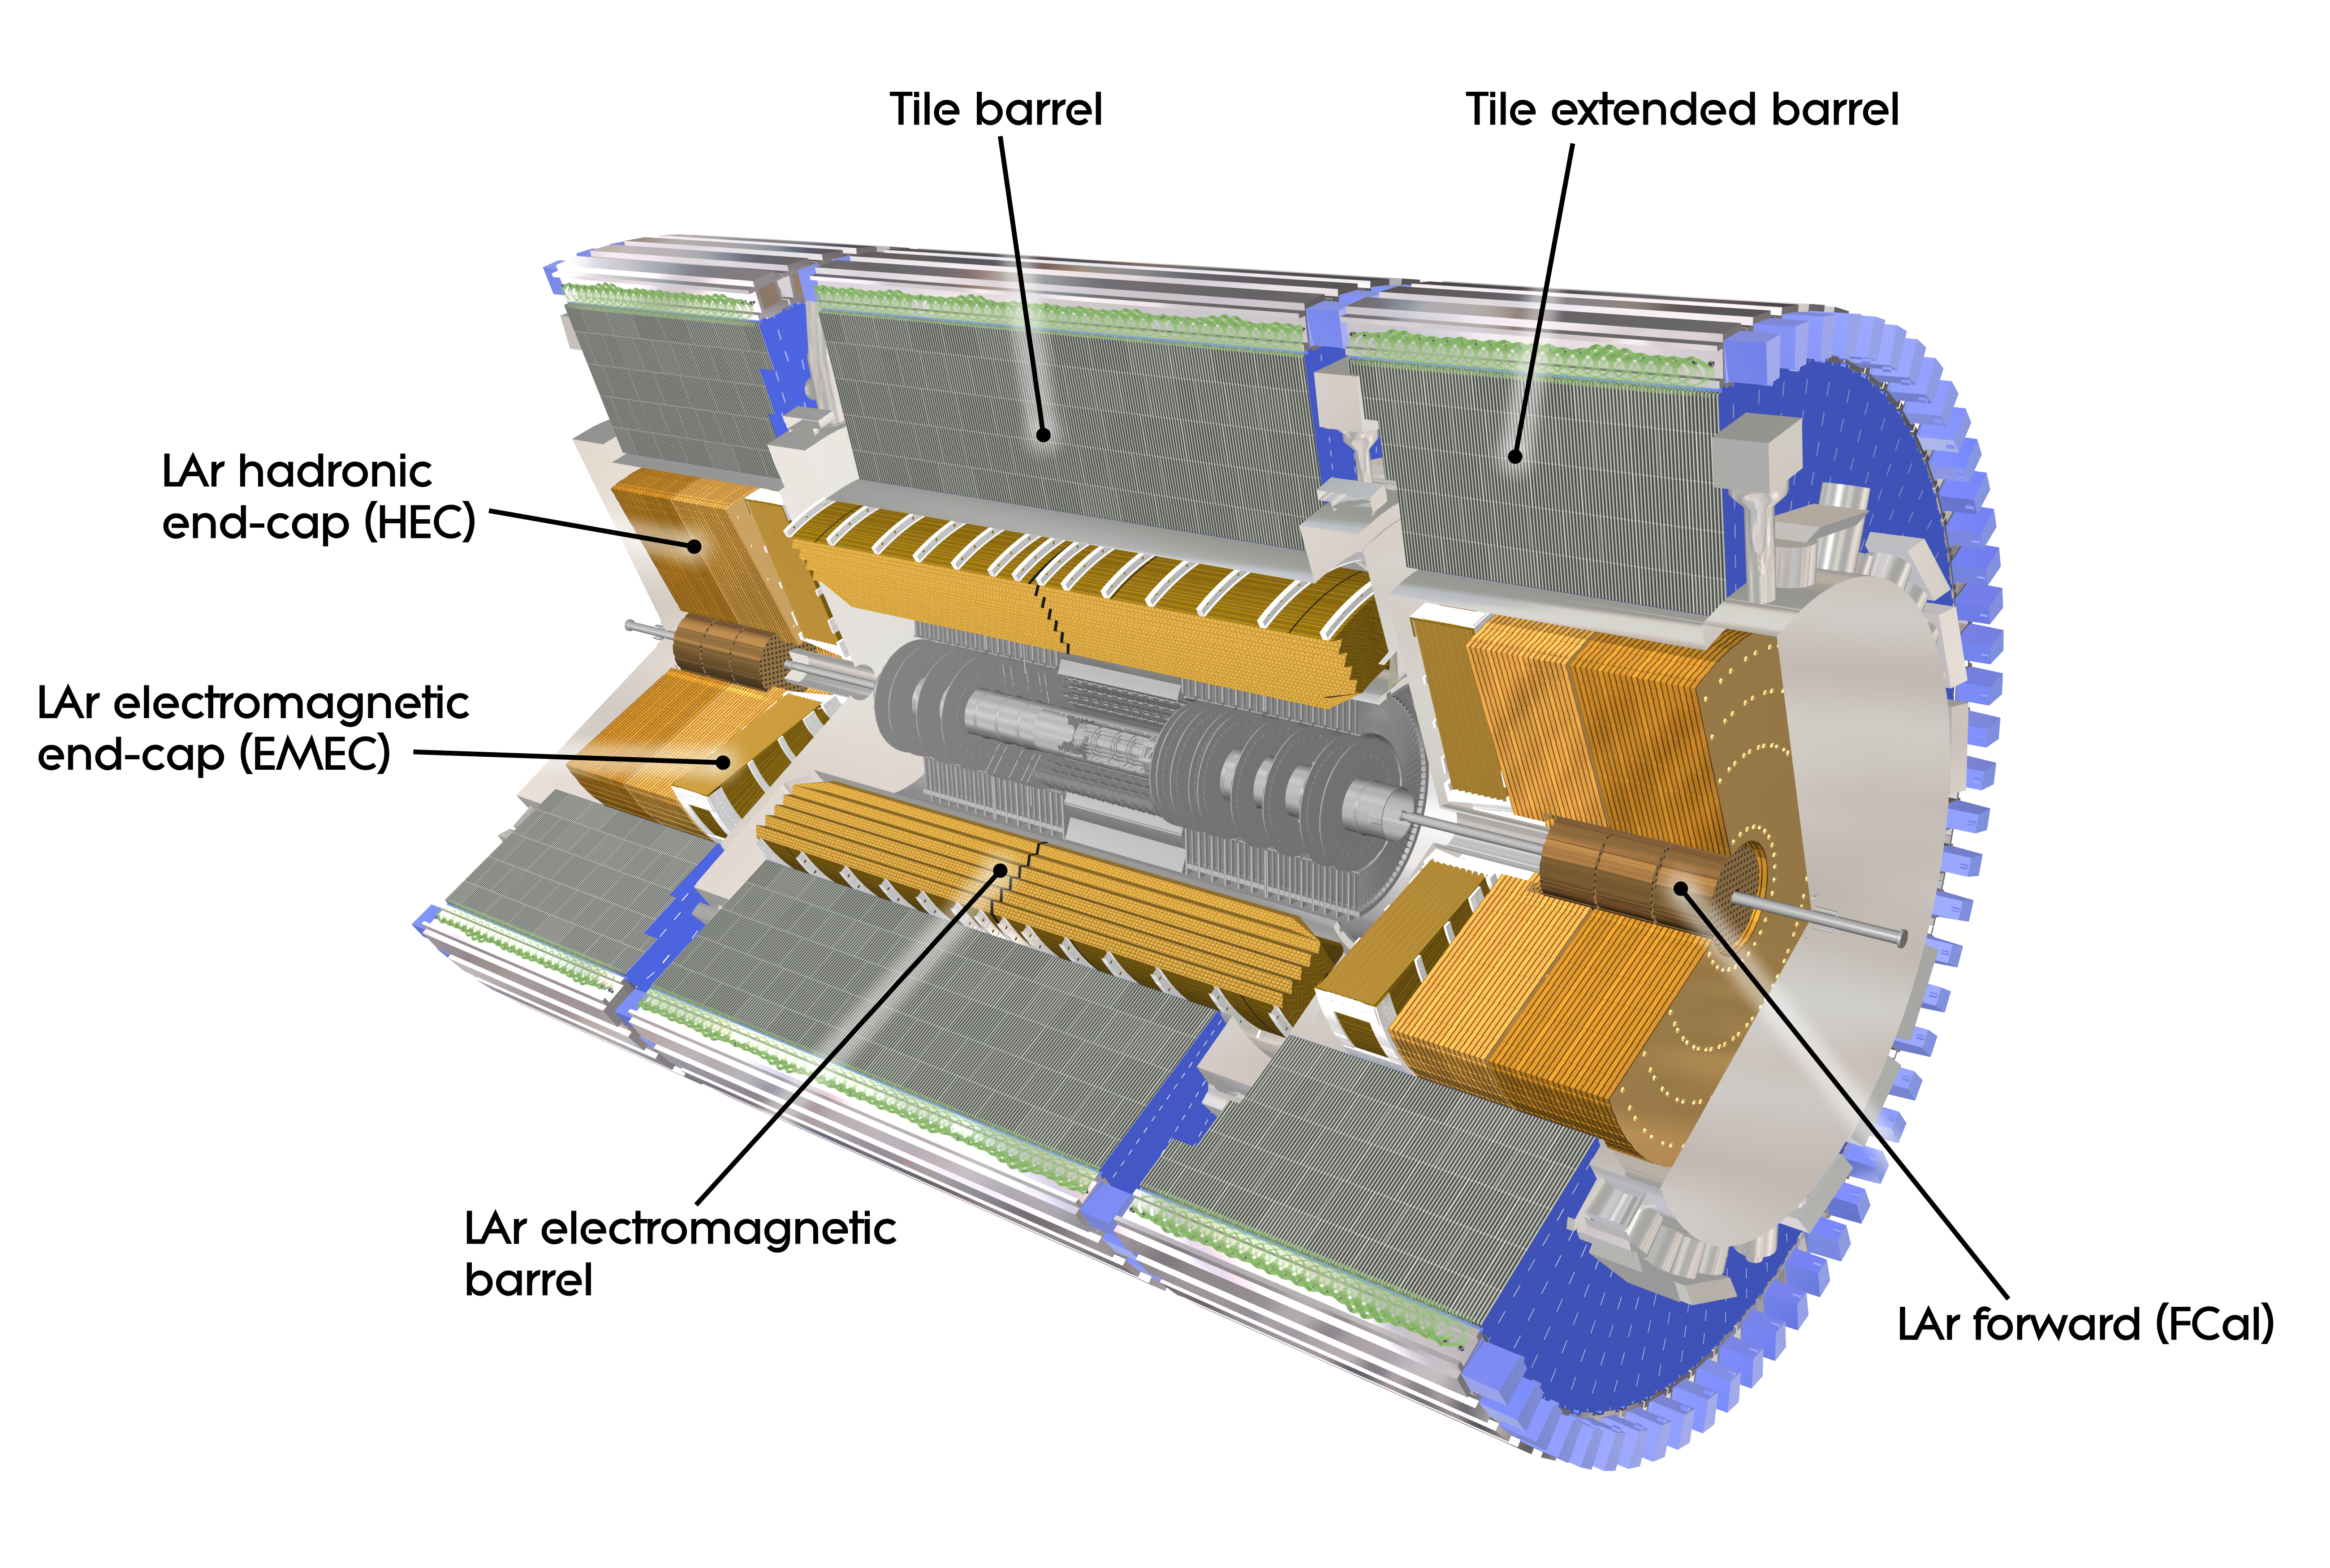
\includegraphics[width=0.7\textwidth]{figures/atlas-detector/0803015_01.jpg}
    \caption{Computer generated image of the \atlas calorimeter (\copyright\ \cern).}
    \label{fig:colorimeter}
\end{figure}\noindent
The calorimeters are the detector layers following the inner detectors. Its structure is divided into the Electromagnetic calorimeter (ECal) and the hadronic calorimeter (HCal).
\subsubsection{Electromagnetic Calorimeter}
The ECal is used for the energy and position measurement of electric charged particles and photons. It utilizes bremsstrahlung and pair production to create a cascade of charged particles which are measured. It offers full azimuthal coverage and is equipped with end caps in the longitudinal direction of the beam pipe. The \atlas ECal is a sampling calorimeter operating with lead as the passive and liquid Argon as the active medium. The innermost part of the ECal is a presampler which detects if the particle started showering before reaching the ECal.
\subsubsection{Hadronic Calorimeter}
The HCal measures the energy and position of baryons and mesons through strong interactions with the nuclei. In the range of $|\eta|<1.7$ it is a sampling calorimeter with steel as the passive and scintillators as the active medium. For the end cap, liquid Argon is deployed as the active medium. The HCal works with the same principle as the ECal but offers less precise measurements.

In the range of $3.1<|\eta|<4.9$ ECal and HCal are substituted with the forward calorimeters (FCal) which are made up of three modules to fulfil the function of both calorimeters.

In combination with the FCal a total range of $|\eta|<4.9$ is covered by the calorimeters.

A computer-generated image of the structure of the different calorimeters used in the \atlas detector is shown in \Cref{fig:colorimeter}.
\subsection{Muon Spectrometer}
The muon spectrometer is the outermost part of the \atlas detector. Its purpose is to detect charged particles exiting the calorimeters and measure their momentum in the range of $|\eta|<2.7$. A detector dedicated to the measurement of muons is necessary because their mass makes them minimal ionizing particles in the energy range of the \lhc collisions. The amount of energy loss due to bremsstrahlung is not sufficient to develop showers necessary to measure their energy. The muons' transverse momenta can be measured in the ID. Like the inner detector, the muon spectrometer utilizes a magnetic field to conduct a measurement of the particle's momentum.  In the muon spectrometer, however, a solenoid magnet is used to allow for the measurement of the muon's momentum along a different direction. Combining the measurements, one obtains full knowledge of the muons four-momentum. Further, does the high rate of stopped electrons and hadrons in the calorimeters enable a high specificity in the muon detection.


\subsection{Trigger System}
With a bunch spacing of $25\,\unit{\nano\second}$ \cite{ATLAS:2019pzw} collisions happen at a rate of $40\,\unit{\mega\hertz}$. Each collision involves up to hundreds of particles. To reduce the data to a feasible amount, triggers are employed to filter less interesting events. Different layers of triggers operate either at the hardware or software level. The L1 trigger is a hardware level trigger and acts as the first filter for the events. It makes decisions in less than $2.5\,\unit{\micro\second}$. The subsequent L2 trigger is a software level trigger and makes decisions in less than $200\,\unit{\micro \second}$. Combined, the trigger system reduces the event rate from $40\,\unit{\mega\hertz}$ to $1000\,\unit{\hertz}$ which are then stored at the \cern data centre.



\appendix
\chapter{Additional Plots}



\cleardoublepage


\bibliography{bthesis_datenbank} 

\chapter*{Danksagung}
Dank\dots

\begin{otherlanguage}{ngerman}
\Declaration
\end{otherlanguage}
\end{document}
